\chapter{\hspace*{3pt} Ciências Cognitivas}

Neste capítulo vamos discorrer de maneira breve sobre as principais áreas que discutem a possibilidade de aquisição do conhecimento pelo homem, assim como a sua representação.

Dado este propósito, parece impossível não tanger a área das ciências cognitivas, área interdisciplinar que, segundo \citeonline{lacerda:2012.linguagem}:
\begin{quote}
[...]descreve, explica, e, eventualmente, simula as principais disposições e capacidades da cognição humana: a linguagem, a percepção, a coordenação motora e a planificação, objetivando entender a aquisição de conhecimentos ou das percepções dos seres humanos e de seus processos mentais \cite{lacerda:2012.linguagem}.
\end{quote}
\apudonline{casti:1989.paradigms}{saracevic:2008.ciencia} define Ciência Cognitiva como a ``[...] amálgama de psicologia, filosofia, antropologia, neurofisiologia, ciência da computação e linguística, organizada em torno do uso do computador enquanto ferramenta capaz de extrair os segredos da mente”.

O hexágono cognitivo, Figura 1, mostra como se daria o relacionamento entre essas áreas, destacando a natureza de seu vínculo, isto é, as disciplinas que possuem um forte vínculo interdisciplinar, representado pelas linhas fortes, e as que possuem vínculo interdisciplinar fraco, representado pelas linhas tracejadas \cite{lacerda:2012.linguagem}.

\begin{figure}
    \centering
    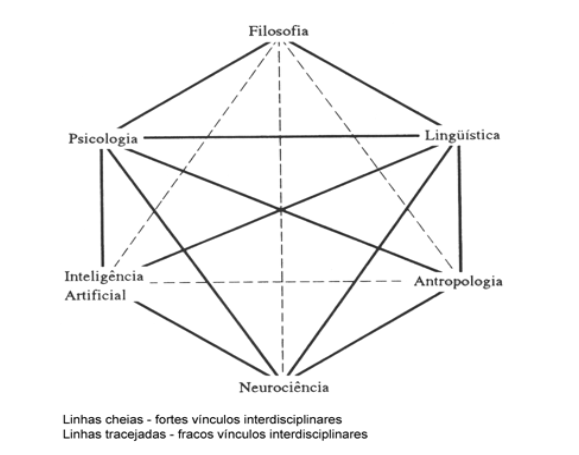
\includegraphics[width=\textwidth]{imagens/hexagono_cognitivo.png}
    \caption{Relações entre as Ciências Cognitivas. Fonte: \apudonline{gardner:1995.nova}{lima:2003.interfaces}}
    \label{fig:hexagono_cognitivo}
\end{figure}

Neste trabalho, por uma questão de redução de escopo, nos ocuparemos principalmente pelo seu forte vínculo interdisciplinar e discurso associativo com o tema proposto para investigação, das áreas da Filosofia, Psicologia e Linguística, através das teorias que dão fundamentação a esta dissertação.

\section{\hspace*{3pt} Conhecimento}

Com o advento da escrita, e até antes disto, com as representações pictográficas, ao homem foi possível romper as limitações de sua própria existência para a preservação do conhecimento. A representação do conhecimento, é desta maneira, o ponto determinante do processo informacional, visto que recai sobre ela a tarefa de manifestar o saber sobre seres e as coisas do mundo real para aquele que será o usuário final da informação \cite{caixeta:2008.representacao}.

Tão importante quanto sua representação, o que podemos definir como sendo conhecimento, e o que possibilita ao homem adquiri-lo desperta a atenção dos estudiosos, desde a Grécia antiga.

De maneira bem ampla, podemos definir conhecimento como a relação entre o sujeito e o objeto, onde a função do sujeito é apreender o objeto e a função do objeto é ser apreensível e ser apreendido pelo sujeito, com a finalidade de dominá-lo e utilizá-lo para entendimento e elucidação da realidade.

As questões acerca da possibilidade de conhecer, no entanto, apresentam diferentes correntes e teorias. No campo da Filosofia, o criticismo propõe que o conhecimento só é possível devido a sensibilidade que dá à matéria do saber e ao entendimento, que dá às formas do conhecimento, sendo esta uma teoria intermediária entre a teoria empirista e a teoria racionalistas \cite{kant:1983.critica}.

A sensibilidade nos fornece intuições, representações singulares que se referem imediatamente aos objetos particulares, e o entendimento produz conceitos, representações gerais que se referem sempre a outras representações(imediatamente aos objetos) \cite{pereira:2011.espaco}.

Geralmente o vocábulo conceito é usado para referir-se a uma unidade do conhecimento (Gercina Ângela Borém Lima, 2007). Segundo o dicionário online Priberam, (2015), o termo “conceito” tem origem na palavra latina “conceptus” (do verbo concipere) que pode ser traduzida como “coisa concebida” ou “formada na mente”, e pode significar, entre outros: 1. Concepção compreendida numa palavra que designa características e qualidades de uma classe de objetos, abstratos ou concretos; 2. Opinião ou ideia, juízo que se faz de alguém ou de alguma coisa; 3. Expressão sintética.

Conceito é uma noção abstrata, uma representação mental referenciada em cada palavra de uma língua que corresponde a um conjunto de propriedades comuns a um grupo de seres - reais ou abstratos - ou objetos, determinando como as coisas são.

De acordo com Paul Thagard; Ethan Toombs, (2005), essas representações mentais, geralmente, correspondem e se referem a classes de coisas do mundo.

2.2. Linguística

Dahlberg preocupada com a compreensão da importância do conceito, na representação do conhecimento, explicita o estudo sobre conceitos na Ciência da Informação (Nonatto, Rafael dos Santos, 2009). A teoria do conceito busca uma base mais sólida para determinar e entender o que consideramos como um conceito (Campos, Maria Luiza de Almeida, 2001).

A autora apresenta ainda o triângulo semântico de Ogden e Richards (Ogden, Charles Kay et al., 1923), Figura 2, que serve como modelo para construção de conceitos, e onde estão representadas as relações entre o objeto ou o referente, o conceito ou o pensamento/referência e o termo ou símbolo.


Triângulo Semiótico.

Sabemos que o homem tem a capacidade de fazer afirmações sobre as coisas reais e sobre ideias que existem apenas em sua mente, através das linguagens naturais, linguagens utilizadas nas necessidades da vida cotidiana (Campos, Maria Luiza de Almeida, 2001).

Essas afirmações, ou enunciados, podem falar a respeito de objetos da sensibilidade ou de objetos do entendimento, de maneira geral ou de maneira individuais. Os objetos gerais são aqueles que estão situados fora de um espaço e um tempo específico, um contexto, e constituem-se de enunciados mais genéricos. Os objetos individuais, por outro lado, podem ser pensados como exclusivos e distintos dos demais, isto é, constituem uma unidade inconfundível. Por exemplo, podemos falar sobre Clint Eastwood ou sobre atores do cinema Western, para exemplificar conceitos específicos ou gerais, respectivamente (Dahlberg, Ingetraut, 1978; Dahlberg, Ingetraut, 1978).

Na teoria proposta por Dahlberg, as características desempenham um papel fundamental. Ela define um conceito como uma série de enunciados, isto é, características verdadeiras sobre um objeto, reunidos de maneira sintética, sob uma ``tag'', um signo capaz de representar essa síntese.

Dahlberg também faz uma distinção importante entre unidade do pensamento e unidade de conhecimento. Segundo ela, a unidade de pensamentotransmite uma ideia de subjetividade enquanto a unidade de conhecimentoremete a um entendimento objetivo. A figura 3, representa os três passos envolvidos na formação de um conceito (Campos, Maria Luiza de Almeida, 2001).


Modelo para Construção de Conceitos em Dahlberg.
No momento em que selecionamos um objeto, tem-se início o processo de determinação de um conceito. Atribuímos predicados a este objeto, destacando as suas características mais relevantes. ParaIngetraut Dahlberg, (1978), as características relevantes são aquelas necessárias para queo objetoseja exatamente ele e não outro. Essas característicasauxiliam o processo de designação do objeto, e a junção destas característicasdevem ser expressas ou representadas por um signo.

Nossa comunicação, designando os objetos que estão ao nosso redor e transmitindo os pensamentos, que somos capazes de formular em nossos íntimos, sobre esses mesmos objetos só nos é possível graças à linguagem; a princípio um conjunto de símbolos pictográficos, que ganharam regras e representações sonoras, originando a fala e a escrita (Dahlberg, Ingetraut, 1978).

Desde a nossa infância, fomos habituados aassociar os objetos asons e sinais pré-determinados. Tornando-se natural, no decorrer de nossas vidas, que nossa percepção trabalhe com representações icônicas (figuras e imagens), um mundo visual que está ao nosso redor(Engelkamp, J., 1976)apud(Dahlberg, Ingetraut, 1978). REVER

2.3. Filosofia

A preocupação em nomear, definir e categorizar as coisas do mundo é antiga e passou de um processo individual a um processo cultural e social. Lima, Gercina Ângela Borém, (2007), em consonância com outros autores, considera os termos categorização e classificação como sinônimos.

Categorização ou classificação é o processo cognitivo de dividir as experiências do mundo em grupos de entidades ou categorias, para construir uma ordem física e social do mundo (Lima, Gercina Ângela Borém, 2003). Na concepção dada por Iyer, Hemalata, (1995), as categorias concedem estabilidade e ordem ao mundo que percebemos, segmentando-o, possibilitando agrupamentos de objetos de formas utilizáveis, nesse sentido, torna-se impossível pensar sem formar categorias (Artêncio, Luciane Maria, 2012).

A categorização, segundo Silva, Alessandra Rodrigues da; Lima, Gercina Ângela Borém, (2011), é o processo cognitivo de compreensão das características dos objetos por critérios de similitude ou diferença. Entretanto, Artêncio, Luciane Maria, (2012)argumenta que atualmente a categorização não vem recebendo a atenção que lhe é necessária nos estudos desenvolvidos na Ciência da Informação:

Ainda que contemporaneamente a categorização seja assumida, ou como parte da capacidade intelectual necessária ao ser humano para a efetivação do processo cognitivo, ou como expressão sócio-cultural de organizar o mundo, de um modo geral, ela não tem sido reconhecida como uma questão presente nos discursos da Ciência da Informação (Artêncio, Luciane Maria, 2012).
Aranalde, Michel Maya, (2009),em um tratamento contemporâneo e com respaldo da filosofia e da teoria da classificação, defende:

As categorias são identificadas como conceitos elementares, isto é, como princípios que permitem identificar as notas essenciais que caracterizam um objeto de conhecimento. A partir desta operação mental de identificação, é possível formular conceitos empíricos, ou seja, buscar uma equivalência entre como o objeto se apresenta e a representação mental que se faz dele e de suas relações com outros objetos. As categorias são concebidas como meta-conceitos que permitem a efetiva conceitualização de objetos passíveis de serem conhecidos, organizados e classificados. Portanto, elas são elementos intermediários entre os conceitos e a realidade cognoscível(Aranalde, Michel Maya, 2009).
Blair, David, (2006) concebe as categorias como a base da linguagem. A categorização, sob sua perspectiva, é uma forma de simplificação que provê um sistema de referência básico no qual coisas que são fundamentalmente diferentes são tratadas como se fossem semelhantes(Artêncio, Luciane Maria, 2012).

A capacidade de listar as características do objeto percebido e compará-las a de outros objetos já conhecidos, é um privilégio da racionalidade humana, que permitem a percepção, classificação e criação de conhecimentos acerca dos objetos(Alvarenga, Lídia, 2003).

A organização do conhecimento, da sua representação à sua recuperação, está estritamente relacionada com os conceitos que compõemo campo do saber abordado e as relações entre eles, tendo em mente a influência do contexto, em qualquer descrição e representação individual dos mesmos(Lima, Gercina Ângela Borém, 2003).

Corroborando com esta ideia,Mauss, Marcel, (1999) , explica que existe um relação estreita entre os sistemas sociais e suas relações lógicas, reforçando a ideia de que em torno de um signo, em sua representação ampla, existe a participação coletiva e social, fruto de um arranjo semântico de uma comunidade, de uma raça, de uma sociedade(Artêncio, Luciane Maria, 2012).

Com a linguística, a categorização passou a ser encarada por outro viés, se ocupar dos métodos utilizados pelos sujeitos para categorizar, descrever, justificar, compreender os fenômenos da vida cotidiana(Jan Edson Rodrigues-Leite, 2005).

2.4. Psicologia

A psicologia, apresenta algumas teorias para a construção do conhecimento. Piaget, por exemplo, defende que a representação funciona através de signos, que durante a construção do conhecimento são associados a imagens mentais, o que permite sua evocação posterior, em outro objeto ou atividade(Smolka, Ana Luiza B, 1993).

O modelo de protótipo, defende que conceitos são representados por um grupo de características, e não por suas definições. O agrupamento de conceitos em uma dada categoria se daria, segundoRosch, Eleanor, (1999), não pela alternância dos traços dicotômicos, mas pela semelhança com o protótipo, em que um membro condensasse os traços mais característicos da categoria.

O pilar desta teoria, sustenta que as categorias são organizadas em torno de protótipos centrais, isto é, um exemplo representativo de uma categoria seria aquele que compartilhasse com os outros membros de sua categoria o maior número de características e que, por outro lado, compartilhasse de poucas características, ou nenhuma, com elementos de fora desta(Lima, Gercina Ângela Borém, 2007).

Rosch, Eleanor, (1999), propõe uma série de experimentos onde comprova que existem dois princípios gerais e básicos para formação de categorias. O primeiro afirma que a tarefa dos sistemas de categoria é fornecer o máximo de informação com o menor esforço cognitivo, princípio que ela denomina como economia cognitiva (tradução livre de Cognitive Economy); o segundo afirma que o mundo percebido se apresenta através de informações estruturadas em vez de atributos arbitrários ou imprevisíveis, princípio nomeado de estrutura do mundo percebido (tradução livre de Perceived World Structure).

Esses dois princípios, combinados, implicam para o nível de abstração de categorias formadas em uma cultura e para a estrutura interna das categorias, se apresentando em duas dimensões: a vertical e a horizontal (Rosch, Eleanor, 1999).

A dimensão verticalintroduz o conceito de objetos de nível básico, diz respeito a capacidade de inclusão de uma categoria, isto é, qual categoria é mais abrangente e qual é menos. A dimensão horizontal diz respeito à segmentação de categorias no mesmo nível de inclusividade. Como uma categoria se organiza internamente, ou seja, temos categorias distintas, dentro do mesmo grau de inclusão. A Figura 4demonstra níveis de categorização nas duas dimensões e apresenta alguns exemplos (Lacerda, Naziozenio Antonio, 2012).

Níveis de Categorização
Como podemos ver, as dimensões demonstram que o nível básicoé o nível mais equilibrado, ou seja, é o nível onde os conceitos são mais expressivos e há uma maior economia cognitiva, isto é, um resumo dos atributos importantes que distinguem uma categoria da outra.
